\documentclass[10pt]{article}

\def\Type{LessonDJ}
\def\TypeNum{Workshop Week 2} %Lesson #
\def\TypeTitle{Limits and Continuity } %Lesson Title
\def\Semester{Fall 2021} %Not Used 
\def\Course{MATH 1190}%Course number and name
\def\Targets{ \target{L1} }

\usepackage{preambleDJ} 

%%%%%%%%%%%% BEGIN DOCUMENT %%%%%%%%%%%%%%%
%%%%%%%%%%%% BEGIN DOCUMENT %%%%%%%%%%%%%%%
%%%%%%%%%%%% BEGIN DOCUMENT %%%%%%%%%%%%%%%
%%%%%%%%%%%% BEGIN DOCUMENT %%%%%%%%%%%%%%%
%%%%%%%%%%%% BEGIN DOCUMENT %%%%%%%%%%%%%%%

\begin{document}
\pagestyle{otherpages}
\thispagestyle{firstpage}

\vs{.5}
{\exercise{\target{L1}}
\enum{

{\exercise{\target{L1}} The graph of the function $f$ is shown below. Use the graph to estimate the values of the following limits. \\
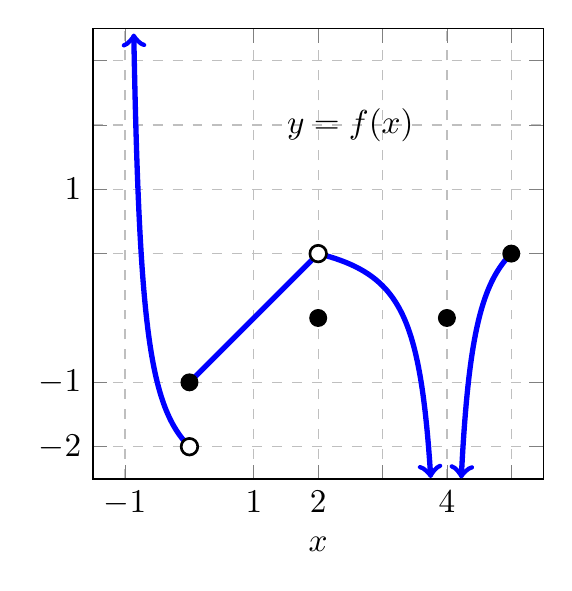
\begin{tikzpicture}[scale=1.2]
  \begin{axis}[
    xlabel={$x$},
    xtick       = {-1,1,2,3,4,5},
    xticklabels = { $-1$, $1$,$2$, ,$4$,},
    ytick       = {-2,-1,1,2,3,4},
    yticklabels = {$-2$,$-1$, ,$1$, , ,},
    samples     = 320,
    domain      = -2.5:5.5,
    restrict y to domain=-2.5:4.5,
    xmin = -1.5, xmax = 5.5,
    ymin = -2.5, ymax = 4.5,
    width = 2.5in, height = 2.5in,
    grid=both, grid style=dashed
  ]
  \node at (2.5,3) {$y=f(x)$};
  % pieces 1 & 2
  \addplot[domain=-1:0, blue, ultra thick, mark=none, <-] {-3+1/(x+1)};
  \draw[blue, ultra thick] (0,-1) -- (2,1);
  \filldraw[white] (0,-2) circle (2.5pt);
  \draw[thick] (0,-2) circle (2.5pt);
  \filldraw (0,-1) circle (2.5pt);
  \filldraw (2,0) circle (2.5pt);
  % piece 3
  %\addplot[domain=2:3, blue, ultra thick, mark=none] {(x-3)^3+2};
  \addplot[domain=2:4, blue, ultra thick, mark=none, ->] {1/(x-4)+1.5};
  \filldraw[white] (2,1) circle (2.5pt);
  \draw[thick] (2,1) circle (2.5pt);
  % piece 4
  \addplot[domain=4:5, blue, ultra thick, mark=none, <-] {-1/(x-4)+2};
  %\addplot[domain=4:5, blue, ultra thick, mark=none] {-7*(x-5)^7+1};
  \filldraw (4,0) circle (2.5pt);
  \filldraw (5,1) circle (2.5pt);
\end{axis}
\end{tikzpicture}

\begin{enumerate}
\item[(a)] $\displaystyle\lim_{x\to0^-} f(x)=$ \\ 
\item[(b)] $\displaystyle\lim_{x\to0^+} f(x)= $
\item[(c)] $\displaystyle\lim_{x\to0} f(x)= $ 
\item[(d)] $\displaystyle\lim_{x\to2^-} f(x)= $ 
\item[(e)] $\displaystyle\lim_{x\to2^+} f(x)= $ 
\item[(f)] $\displaystyle\lim_{x\to2} f(x)=$ 
\end{enumerate}

\begin{enumerate}
\item[(g)] $\displaystyle\lim_{x\to4^-} f(x)=  $  \\
\item[(h)] $\displaystyle\lim_{x\to4^+} f(x)=  $  \\
\item[(i)] $\displaystyle\lim_{x\to4} f(x)=  $  \\
\item[(j)] $\displaystyle\lim_{x\to-1^+} f(x)=  $  \\
\item[(k)] $\displaystyle\lim_{x\to1} f(x)=  $  \\
\end{enumerate}
\newpage
{\exercise{\target{L1}} 
\enum{
\item[E1.] In terms of limits, what does it mean for $f$ to have a removable discontinuity at $x=a$?

\vfill

\item[E2.] In terms of limits, what does it mean for $f$ to have a jump discontinuity at $x=a$?

\vfill

\item[E3.] In terms of limits, what does it mean for $f$ to have an infinite discontinuity at $x=a$?

\vfill

}

\end{document}